\documentclass[11pt,a4paper]{article}

\usepackage[utf8]{vietnam}
\usepackage[a4paper, margin=2cm]{geometry}
\usepackage{amsmath,amssymb}
\usepackage{booktabs}
\usepackage{enumitem}
\usepackage{tabularx}
\usepackage{longtable}
\usepackage{array}
\usepackage{graphicx}
\usepackage{float}
\usepackage{caption}
\usepackage{subcaption}
\usepackage[hyphens]{url}
\usepackage[hidelinks]{hyperref}

\setlength{\parindent}{0pt}
\setlength{\parskip}{4pt}
\urlstyle{same}
\setlist{nosep, topsep=2pt, itemsep=2pt}
\captionsetup{skip=4pt}
\captionsetup[subfigure]{skip=3pt}

\renewcommand{\topfraction}{0.9}
\renewcommand{\bottomfraction}{0.8}
\renewcommand{\textfraction}{0.07}
\renewcommand{\floatpagefraction}{0.85}

\newcolumntype{L}[1]{>{\raggedright\arraybackslash}p{#1}}
\newcolumntype{C}[1]{>{\centering\arraybackslash}p{#1}}
\newcolumntype{Y}{>{\raggedright\arraybackslash}X}

\begin{document}

% =========================================================================
% PHẦN ĐẦU TRANG: THÔNG TIN SINH VIÊN & TIÊU ĐỀ
% =========================================================================
\begin{center}
    {\large \textbf{ĐẠI HỌC QUỐC GIA THÀNH PHỐ HỒ CHÍ MINH}}\\[0.2em]
    {\large \textbf{TRƯỜNG ĐẠI HỌC KHOA HỌC TỰ NHIÊN}}\\[0.3em]
    {\normalsize \textbf{KHOA CÔNG NGHỆ THÔNG TIN -- CHƯƠNG TRÌNH TIÊN TIẾN (APCS)}}\\[1.0em]

    \hrule height 0.8pt
    \vspace{0.5em}
    {\Large \textbf{BÁO CÁO THỰC NGHIỆM KIỂM THỬ CÔNG CỤ AI}}\\[1.4em]
    \hrule height 0.8pt
\end{center}

\vspace{0.2em}
\begin{tabularx}{\textwidth}{@{}L{4cm}Y@{}}
    \textbf{Họ và tên:} & Đỗ Viết Hoàng Long \\
    \textbf{MSSV:} & 25125024 (Lớp: 25A01) \\
    \textbf{Môn học:} & Phương pháp Nghiên cứu Khoa học (SC203) \\
    \textbf{Công cụ kiểm thử:} & Google Cloud Vision API\\
\end{tabularx}
\vspace{0.2em}
\hrule
\vspace{0.5em}

% =========================================================================
% SECTION 1: GIỚI THIỆU CÔNG CỤ AI & PHÁT BIỂU GIẢ THUYẾT
% =========================================================================
\section{Giới thiệu Công cụ AI \& Phát biểu Giả thuyết}

\subsection{Giới thiệu Công cụ và Vấn đề Nghiên cứu}
Google Cloud Vision API là dịch vụ nhận dạng ký tự hoạt động theo quy trình hai giai đoạn: 

\begin{itemize}
	\item[(1)] Phát hiện vùng chứa văn bản bằng hộp giới hạn (\textit{Bounding Box}).
	\item [(2)] Nhận dạng chuỗi ký tự kết hợp mô hình ngôn ngữ. Mặc dù công cụ này hoạt động ổn định trên văn bản in tiêu chuẩn, việc nhận dạng tiếng Việt trong thực tế gặp nhiều thách thức do hệ thống dấu thanh và dấu phụ phức tạp (\textit{ă, â, đ, ê, ô, ơ, ư} cùng 5 thanh điệu), đặc biệt khi văn bản được thể hiện dưới dạng chữ thư pháp, chữ cách điệu hoặc chữ viết tay.
\end{itemize}

\subsection{Giả thuyết Nghiên cứu}
Trong báo cáo này, tôi đặt ra giả thuyết nghiên cứu như sau:
\begin{quote}
\textit{``Google Cloud Vision API hoạt động kém hiệu quả hoặc thất bại trong việc bóc tách chính xác văn bản tiếng Việt khi chữ viết có tính nghệ thuật cao (chữ thư pháp Quốc ngữ, chữ viết tay tiểu học nét thanh nét đậm, chữ cách điệu uốn lượn), dẫn đến hiện tượng mất dấu thanh/dấu phụ, phân đoạn sai ký tự (over-segmentation) và ghép nhầm ký tự liền kề thành từ vô nghĩa.''}
\end{quote}

% =========================================================================
% SECTION 2: THIẾT KẾ THỰC NGHIỆM & BẢNG KẾT QUẢ
% =========================================================================
\section{Thiết kế Thực nghiệm \& Bảng Kết quả}

Tôi thu thập bộ dữ liệu gồm 10 mẫu ảnh thực tế bao gồm: chữ viết phấn tiểu học, bảng chữ cái viết hoa cách điệu, chữ thư pháp, chữ thiết kế đồ họa (Typography/Calligraphy), biển báo và chữ viết tay tự nhiên. Các ảnh được đưa vào giao diện kiểm thử của Google Cloud Vision API để đối chiếu kết quả trích xuất với nội dung gốc (Bảng \ref{tab:results}).

{\footnotesize
\renewcommand{\arraystretch}{1.22}
\setlength{\LTpre}{4pt}
\setlength{\LTpost}{4pt}
\begin{longtable}{@{}C{0.7cm} L{2.7cm} L{4.6cm} L{5.7cm} C{1.6cm}@{}}
\caption{Kết quả kiểm thử Google Cloud Vision API trên 10 test case} \label{tab:results} \\
\toprule
\textbf{STT} & \textbf{Loại mẫu (File)} & \textbf{Ground Truth / Input} & \textbf{Output từ Vision API} & \textbf{Đánh giá} \\
\midrule
\endfirsthead

\multicolumn{5}{c}{{\footnotesize \tablename\ \thetable{} -- \textit{Tiếp theo trang trước}}} \\[2pt]
\toprule
\textbf{STT} & \textbf{Loại mẫu (File)} & \textbf{Ground Truth / Input} & \textbf{Output từ Vision API} & \textbf{Đánh giá} \\
\midrule
\endhead

\midrule
\multicolumn{5}{r@{}}{} \\
\endfoot

\bottomrule
\endlastfoot

1 & Bảng chữ đứng tiểu học (\texttt{1.jpg}) &
Tiêu đề \textit{``Mẫu chữ đứng''}; các dòng chữ cái: \textit{``a b c e đ q g r s x''}, \textit{``i t u y v n m p l h''}, \textit{``k th nh ph gh tr ngh''}. &
\textbf{Block 1:} \texttt{``a''} \newline
\textbf{Block 2:} \texttt{``câu chứ đừng''}, \texttt{``bced''} \newline
(Gộp sai khung chữ dòng dưới, mất khoảng trắng). &
Không đạt \newline (Fail) \\
\midrule

2 & Bảng chữ hoa cách điệu (\texttt{2.jpg}) &
Các chữ cái viết hoa trên nền ô ly: \textit{``A Ă Â B C D Đ E''}, \textit{``Ê G H I K L M N''}, \textit{``O Ô Ơ P Q R S T U Ư''}, \textit{``V X Y''}. &
\textbf{Block 1:} \texttt{``A Ã Â B C D D E''} / \texttt{``GHI KLAA''} / \texttt{``O O O P Q R S TU U''} \newline
\textbf{Block 2:} \texttt{``V X U''} (Sót chữ \textit{Ê}, mất dấu phụ). &
Không đạt \newline (Fail) \\
\midrule

3 & Vở ghi bài viết tay (\texttt{3.jpg}) &
Trang vở viết tay môn Ngữ văn (\textit{``Ẩn dụ hình thức...''}, \textit{``Ẩn dụ cách thức...''}), phía trên có đặt thước kẻ nhựa. &
\textbf{Block 1--5:} Đọc đúng chữ in trên thước (\texttt{``200mm''}, \texttt{``ACRYLIC GLASS RULER''}), nhưng vùng chữ viết tay bị tách khung vụn và nhận diện sai. &
Không đạt \newline (Fail) \\
\midrule

4 & Tranh thư pháp Quốc ngữ (\texttt{4.jpg}) &
Chữ chính: \textit{``An Nhiên''}. Câu phụ: \textit{``... mở rộng / tâm ra / lòng thanh thản / An nhiên tự tại / đời thong dong...''}. &
\textbf{Block 1:} \texttt{``fo Milo''} \newline
\textbf{Block 2:} \texttt{``tans ra''} / \texttt{``long thacks than''} / \texttt{``do nhiễm tự tại Ads t hong dong ..''}. &
Không đạt \newline (Fail) \\
\midrule

5 & Biển báo có chữ góc nghiêng (\texttt{5.jpg}) &
Biển báo giao thông; góc trái trên có chữ nghiêng \textit{``HÀNG CÓ SẴN''}; đáy ảnh có số điện thoại liên hệ. &
Không trích xuất văn bản; chỉ trả về nhãn đối tượng \texttt{``Traffic sign (87\%)''}. &
Không đạt \newline (Fail) \\
\midrule

6 & Bảng nét chữ thư pháp (\texttt{6.png}) &
Các bước viết nét cọ thư pháp cho chữ cái \textit{``A''}, \textit{``a''}, \textit{``B''}, \textit{``C''}, \textit{``d''}. &
Không phát hiện được văn bản. Nhận diện nhầm 3 chữ \textit{``A''} thành \texttt{``Bird''} ($77\%, 74\%, 68\%$). &
Không đạt \newline (Fail) \\
\midrule

7 & Chữ thiết kế hình học (\texttt{7.jpg}) &
Chữ cách điệu hình học trên nền vân sóng: \textit{``BODY / ON / THE / MOVE''}. &
\textbf{Block 1:} \texttt{``BODY OV THE''} \newline
(Nhận diện sai \textit{``ON''} $\rightarrow$ \texttt{``OV''}, bỏ sót từ \textit{``MOVE''}). &
Không đạt \newline (Fail) \\
\midrule

8 & Chữ uốn lượn nghệ thuật (\texttt{8.jpg}) &
Chữ Calligraphy có nét kéo dài: \textit{``Font Chữ / Uốn Lượn''}. &
\textbf{Block 1:} \texttt{``Font Chis You Pron''} \newline
(Nhận diện sai toàn bộ các từ tiếng Việt có dấu). &
Không đạt \newline (Fail) \\
\midrule

9 & Thư viết tay trên giấy kẻ ngang (\texttt{9.png}) &
Thư viết tay của bệnh nhân: \textit{``Cộng Hòa Xã Hội Chủ Nghĩa Việt Nam / Độc Lập Tự Do Hạnh Phúc / Định Hóa Ngày 30/7/2025...''}. &
\textbf{Block 1:} \texttt{``for Chu''}; \textbf{Block 2:} \texttt{``Cory Ha Doc Lan WiDo Has Phic e Dink Hoa... this Viet day... cho Bar Sin''}; \textbf{Block 3:} \texttt{``I can''}. &
Không đạt \newline (Fail) \\
\midrule

10 & Bưu thiếp viết tay (\texttt{10.png}) &
Bưu thiếp viết tay trên giấy trơn: \textit{``Thương về Nhuệ để nhớ mình hoài --- hoài, tất cả trâm và tóc hát toàn tự tay mình làm...''}. &
\textbf{Block 1:} \texttt{``Thương về Nhuệ để n hớ mình hoài hoài , rấ t cả Trâm và Tóc hát''}. \textbf{Block 2:} Ký tự tiếng Thái (\texttt{U+0E1B}); các dòng dưới bị sót từ. &
Đạt một phần / Không đạt \\
\end{longtable}
}

% =========================================================================
% SECTION 3: PHÂN TÍCH CHI TIẾT CÁC CA THẤT BẠI ĐIỂN HÌNH
% =========================================================================
\section{Phân tích Chi tiết các Ca Thất bại Điển hình}

Từ kết quả thực nghiệm, tôi phân tích 4 nhóm nguyên nhân kỹ thuật chính dẫn đến lỗi nhận dạng của công cụ:

\subsection{Phân đoạn sai hộp giới hạn (Bounding Box) và bỏ sót ký tự}
Bộ phát hiện văn bản (\textit{Text Detector}) xác định vùng chữ dựa trên mật độ cạnh và khoảng cách đồng đều giữa các ký tự. Khi gặp chữ viết có nét kéo dài hoặc bố cục không chuẩn, bước khoanh vùng gặp lỗi:
\begin{itemize}[label=-]
    \item \textbf{Gộp hoặc tách từ sai (Case 1, Case 10):} Ở Case 1 (Hình \ref{fig:group1}a), chữ \textit{``a''} bị tách thành một khối riêng, trong khi các chữ rời nhau \textit{``b c e đ''} lại bị gộp thành một chuỗi liền \texttt{``bced''}. Ở Case 10, khoảng cách giữa các nét trong cùng một từ viết tay làm API ngắt từ \textit{``nhớ''} thành \texttt{``n hớ''} và \textit{``tất''} thành \texttt{``rấ t''} (\textit{over-segmentation}).
    \item \textbf{Bỏ sót ký tự và vùng chữ (Case 2, Case 6, Case 7):} Ở Case 2 (Hình \ref{fig:group1}b), chữ \textit{``Ê''} đầu dòng thứ hai có nét uốn mảnh tách rời nên nằm ngoài hộp giới hạn của cả dòng. Ở Case 7, từ \textit{``MOVE''} được tạo bởi các vạch sọc đứt đoạn khiến mô hình không nhận diện được biên dạng chữ. Đặc biệt ở Case 6 (Hình \ref{fig:group2}b), các nét cọ thư pháp rời rạc làm bộ phận phát hiện văn bản hoàn toàn không kích hoạt, dẫn đến việc bộ nhận diện vật thể phân loại nhầm chữ \textit{``A''} thành hình con chim (\texttt{``Bird''}).
\end{itemize}

\begin{figure}[!htbp]
    \centering
    \begin{subfigure}[b]{0.48\textwidth}
        \centering
        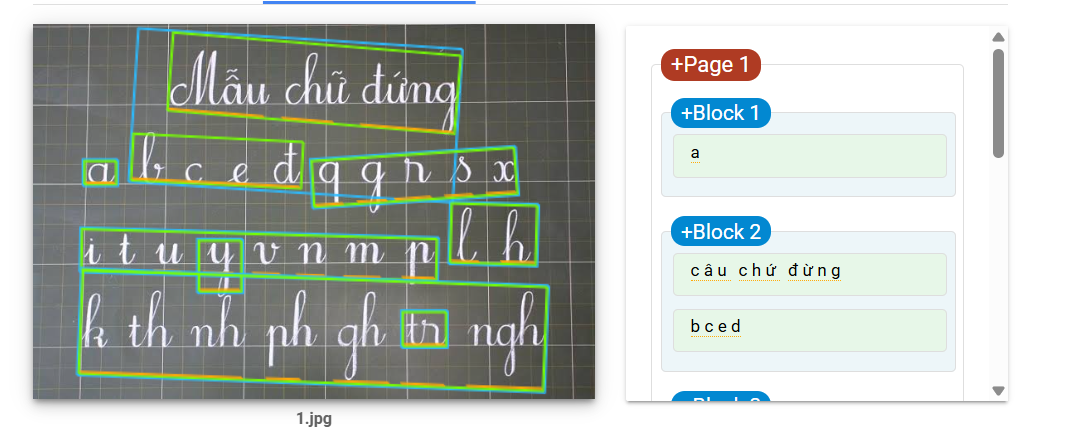
\includegraphics[width=\textwidth, height=3.8cm, keepaspectratio]{TestCase/Output/chrome_HxzYi0QeSz.png}
        \caption{Case 1 (\texttt{1.jpg}): Sai dấu và gộp ký tự \texttt{``bced''}.}
    \end{subfigure}
    \hfill
    \begin{subfigure}[b]{0.48\textwidth}
        \centering
        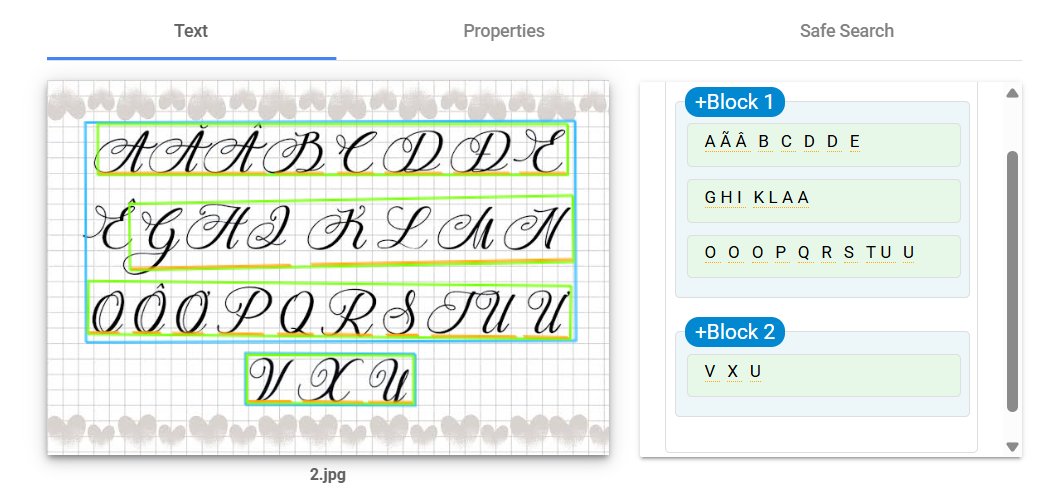
\includegraphics[width=\textwidth, height=3.8cm, keepaspectratio]{TestCase/Output/chrome_HPhhoUtpnw.png}
        \caption{Case 2 (\texttt{2.jpg}): Bỏ sót chữ \textit{Ê} và mất dấu phụ.}
    \end{subfigure}
    \caption{Lỗi khoanh vùng Bounding Box và mất dấu trên chữ mẫu có lưới ô ly.}
    \label{fig:group1}
\end{figure}

\subsection{Mất dấu thanh, dấu phụ và biến dạng nét chữ nghệ thuật}
Đặc trưng nét thanh (mảnh) và nét đậm (dày) của chữ tiểu học hoặc nét cọ thư pháp làm thay đổi hình thái ký tự so với phông chữ in:
\begin{itemize}[label=-]
    \item \textbf{Mất hoặc nhận diện sai dấu tiếng Việt (Case 1, Case 2):} Ở Case 1, cụm \textit{``Mẫu chữ đứng''} bị nhận diện thành \texttt{``câu chứ đừng''} (nét đầu chữ \textit{M} bị lược bỏ, dấu ngã và dấu sắc bị nhận diện sai). Ở Case 2, hầu hết các dấu phụ trên chữ hoa cách điệu bị bỏ qua: \textit{``Ă''} $\rightarrow$ \texttt{``Ã''}, \textit{``Đ''} $\rightarrow$ \texttt{``D''}, \textit{``Ô, Ơ''} $\rightarrow$ \texttt{``O''}, \textit{``Ư''} $\rightarrow$ \texttt{``U''}.
    \item \textbf{Biến dạng cấu trúc chữ cái (Case 2, Case 4):} Các nét uốn vòng vào trong của chữ \textit{``M, N''} hoa ở Case 2 bị đọc nhầm thành \texttt{``AA''}, chữ \textit{``Y''} hoa bị đọc thành \texttt{``U''}. Ở Case 4 (Hình \ref{fig:group2}a), nét cọ lớn của chữ thư pháp \textit{``An Nhiên''} làm chữ \textit{``A''} tách làm hai phần và bị đọc thành \texttt{``fo Milo''}.
\end{itemize}

\begin{figure}[!htbp]
    \centering
    \begin{subfigure}[b]{0.48\textwidth}
        \centering
        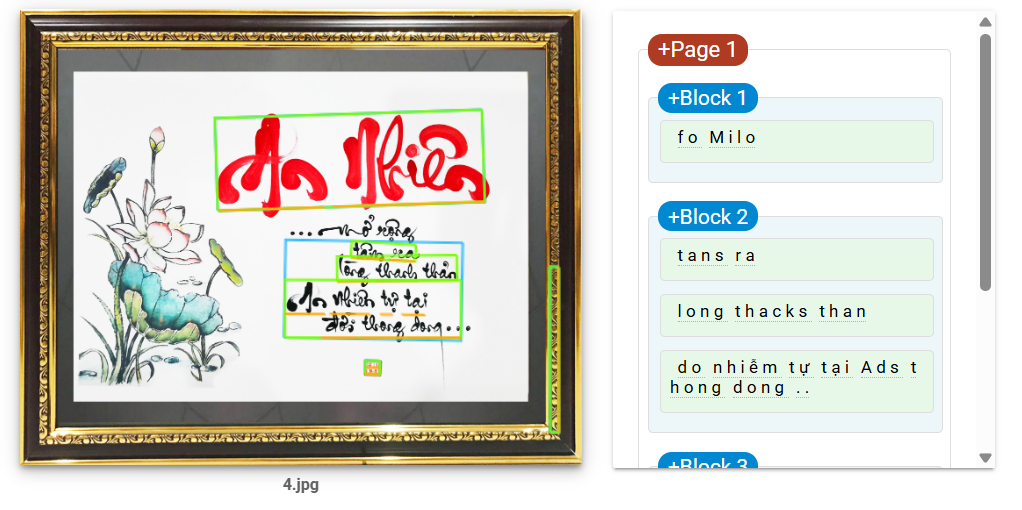
\includegraphics[width=\textwidth, height=4.0cm, keepaspectratio]{TestCase/Output/chrome_Gzv8ovnCzx.png}
        \caption{Case 4 (\texttt{4.jpg}): Chữ thư pháp \textit{``An Nhiên''} $\rightarrow$ \texttt{``fo Milo''}.}
    \end{subfigure}
    \hfill
    \begin{subfigure}[b]{0.48\textwidth}
        \centering
        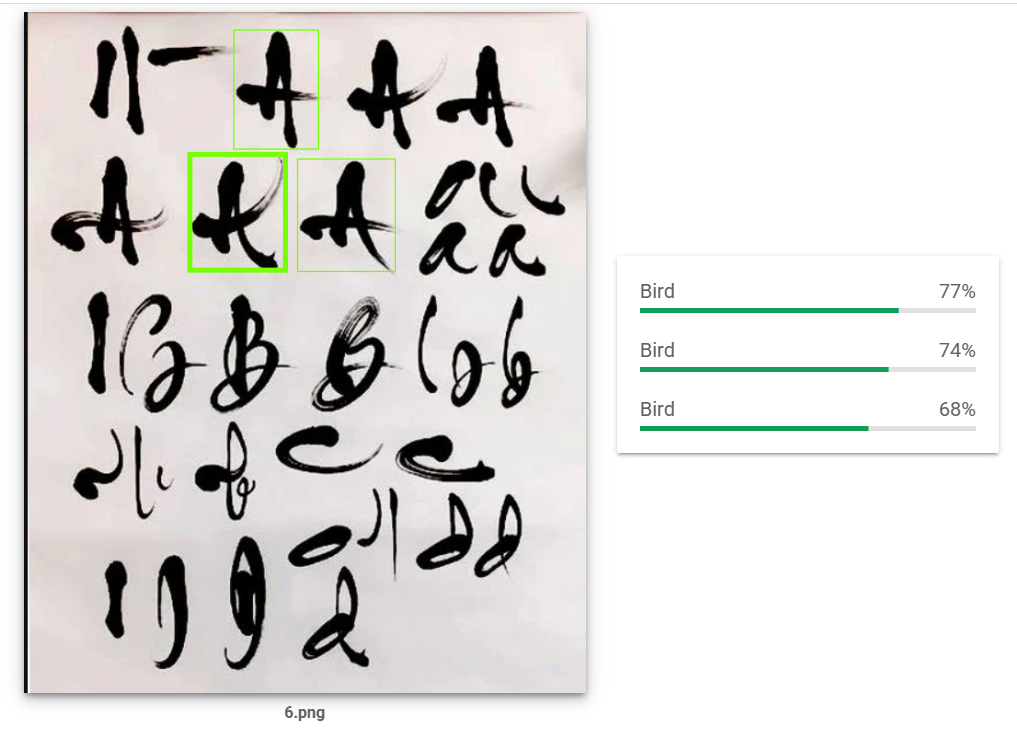
\includegraphics[width=\textwidth, height=4.0cm, keepaspectratio]{TestCase/Output/chrome_MQSShVQNru.png}
        \caption{Case 6 (\texttt{6.png}): Chữ \textit{``A''} thư pháp bị nhận nhầm là \texttt{``Bird''}.}
    \end{subfigure}
    \caption{Lỗi nhận diện trên chữ thư pháp Quốc ngữ.}
    \label{fig:group2}
\end{figure}

\subsection{Ghép nhầm ký tự và thiên lệch sang mô hình ngôn ngữ tiếng Anh}
Khi hình ảnh chữ viết có độ rõ nét thấp hoặc viết nối nét (\textit{cursive}), tầng giải mã ngôn ngữ (\textit{Language Model}) của Vision API có xu hướng ghép các nét chữ thành các từ tiếng Anh thông dụng thay vì từ tiếng Việt:
\begin{itemize}[label=-]
    \item Ở Case 8 (Hình \ref{fig:group3}a), từ \texttt{``Font''} không dấu được đọc đúng, nhưng cụm \textit{``Chữ Uốn Lượn''} có dấu và nét gạch chân uốn cong bị chuyển thành chuỗi từ tiếng Anh không đúng nghĩa gốc là \texttt{``Chis You Pron''}.
    \item Ở Case 9 (Hình \ref{fig:group3}b), văn bản tiếng Việt viết tay của bệnh nhân bị giải mã thành nhiều từ tiếng Anh rời rạc như \texttt{``for Chu''}, \texttt{``this Viet day''}, \texttt{``Bar Sin''} (từ gốc: \textit{Bác Sĩ}), \texttt{``I can''}, \texttt{``this toy''} (từ gốc: \textit{thư tay}).
\end{itemize}

\begin{figure}[!htbp]
    \centering
    \begin{subfigure}[b]{0.48\textwidth}
        \centering
        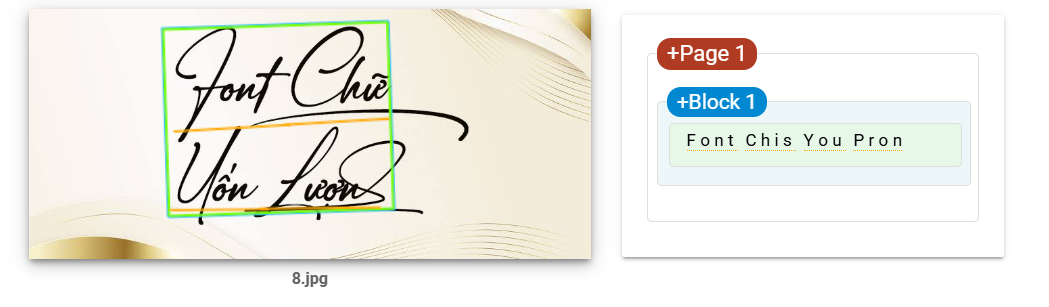
\includegraphics[width=\textwidth, height=4.0cm, keepaspectratio]{TestCase/Output/chrome_3Fxwgqto7f.png}
        \caption{Case 8 (\texttt{8.jpg}): \textit{``Font Chữ Uốn Lượn''} $\rightarrow$ \texttt{``Font Chis You Pron''}.}
    \end{subfigure}
    \hfill
    \begin{subfigure}[b]{0.48\textwidth}
        \centering
        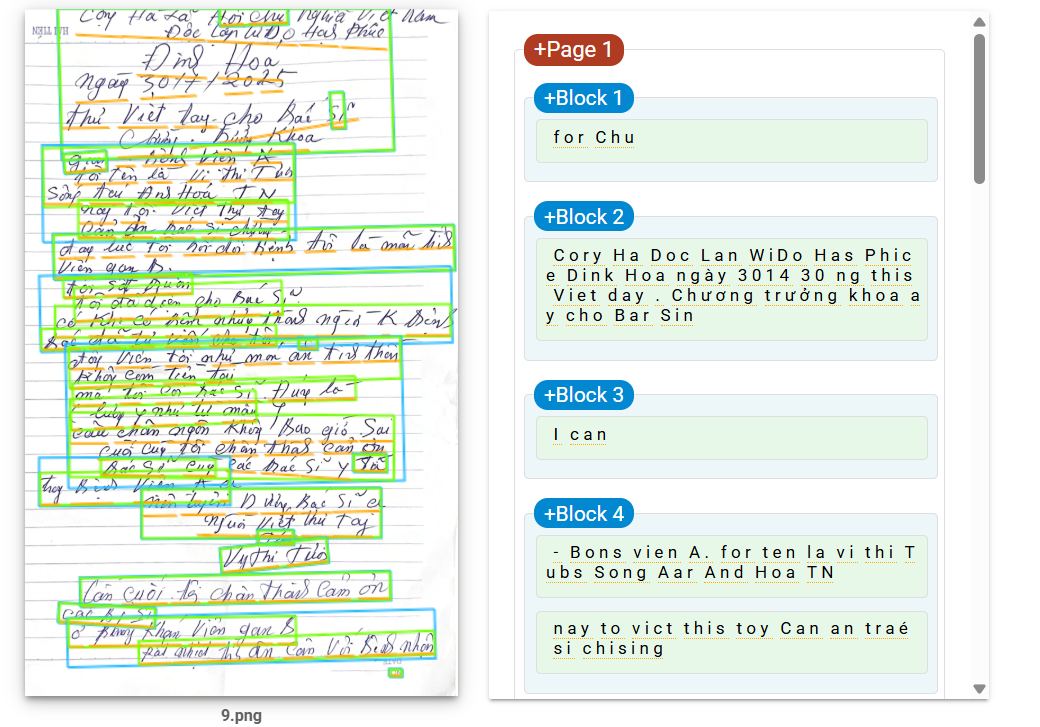
\includegraphics[width=\textwidth, height=4.0cm, keepaspectratio]{TestCase/Output/chrome_GmHf1er7zE.png}
        \caption{Case 9 (\texttt{9.png}): Chữ viết tay tiếng Việt bị chuyển thành từ tiếng Anh.}
    \end{subfigure}
    \caption{Hiện tượng ghép nhầm ký tự sang từ vựng tiếng Anh trên chữ uốn lượn và chữ viết tay.}
    \label{fig:group3}
\end{figure}

\subsection{Ảnh hưởng của nhiễu nền ô ly và dòng kẻ ngang}
Các đường kẻ ô ly trên bảng phấn (Case 1) và dòng kẻ ngang trong vở/giấy viết thư (Case 3, Case 9) cắt ngang qua các nét chữ mảnh và dấu thanh. Ở Case 1, nét gạch ngang của chữ \textit{``đ''} trùng với đường kẻ bảng nên bị loại bỏ thành chữ \texttt{``d''}. Ở Case 3, trong cùng một bức ảnh, API đọc chính xác dòng chữ in trên chiếc thước nhựa (\texttt{``ACRYLIC GLASS RULER''}) nhưng lại khoanh vùng chồng chéo trên phần chữ viết tay có dòng kẻ bên dưới. Ngược lại, ở Case 10 (viết trên giấy trơn không dòng kẻ), dòng đầu tiên được nhận diện tốt hơn đáng kể.

% =========================================================================
% SECTION 4: THẢO LUẬN & KẾT LUẬN
% =========================================================================
\section{Thảo luận \& Kết luận}

\subsection{Kiểm chứng Giả thuyết}
Kết quả thực nghiệm trên 10 test case (9 ca thất bại và 1 ca chỉ đọc đúng một phần câu đầu) \textbf{xác nhận giả thuyết nghiên cứu} đã đề ra. Google Cloud Vision API hoạt động không hiệu quả trên chữ thư pháp Quốc ngữ, chữ viết tay tiểu học nét thanh nét đậm và chữ cách điệu uốn lượn, thể hiện đúng 3 nhóm lỗi dự đoán: mất dấu phụ/dấu thanh, phân đoạn sai hộp giới hạn, và ghép nhầm ký tự thành từ vô nghĩa hoặc từ tiếng Anh.

\subsection{Đánh giá Ưu điểm và Hạn chế của Công cụ}
\begin{itemize}[label=-]
    \item \textbf{Ưu điểm:} Tốc độ xử lý nhanh, nhận diện chính xác các phông chữ in tiêu chuẩn trên nền đồng nhất (như chữ in trên thước kẻ ở Case 3).
    \item \textbf{Hạn chế:}
    \begin{enumerate}[label=(\arabic*)]
        \item Khả năng phát hiện vùng chữ phụ thuộc nhiều vào đường biên ký tự liền mạch, dễ thất bại khi gặp nét cọ thư pháp đứt đoạn hoặc chữ tạo hình học.
        \item Nhạy cảm với nhiễu nền có cấu trúc lặp lại như lưới ô ly bảng phấn và giấy kẻ ngang.
        \item Mô hình ngôn ngữ hậu xử lý chưa tối ưu cho chữ viết tay tiếng Việt, dẫn đến hiện tượng ưu tiên ghép thành từ tiếng Anh khi hình ảnh chữ không rõ ràng.
    \end{enumerate}
\end{itemize}

\end{document}
